%\documentclass[adobefonts]{ctexbook}
\documentclass{ctexbook}
\usepackage{amssymb}
\usepackage{amsfonts}
\usepackage{amsmath}
\usepackage{mathrsfs}
\usepackage{graphicx}
\usepackage{subcaption}
\usepackage{lscape}
\usepackage{afterpage}
\usepackage{diagbox}
%\usepackage{axodraw4j}
\usepackage{pstricks}
\usepackage{color}
\usepackage{txfonts}
\usepackage{media9}
\usepackage{hyperref}
\usepackage[numbers,sort&compress]{natbib}
\usepackage{hypernat}
\usepackage{slashed}
\usepackage{tikz}
\usepackage[overload]{empheq}
\usepackage{relsize}


%\usepackage{theorem}
%\usepackage{ntheorem}
%\usepackage{amsthm}
\usepackage{thmtools}
%\usepackage{showkeys}

\newcommand{\mb}[1]{\mathbf{#1}}
\def\eg{{e.g}. } \def\Eg{{E.g}. }
\def\ie{{i.e}. } \def\Ie{{I.e}. }
\def\cf{{c.f}. } \def\Cf{{C.f}. }
\def\etc{{etc}. }
\def\vs{{vs}. }
\def\wrt{w.r.t. }
\def\dof{d.o.f. }
\def\etal{{et al}. }
\newcommand{\la}{\left\langle}
\newcommand{\ra}{\right\rangle}
\newcommand{\lbar}{\left|}
\newcommand{\rbar}{\right|}
\newcommand{\ldot}{\left.}
\newcommand{\rdot}{\right.}
\newcommand{\st}{\quad s.t. \quad}
\newcommand{\tr}[1]{tr\left(#1\right)}
\newcommand{\rp}{\right)}
\newcommand{\lp}{\left(}
\newcommand{\revision}[1]{{\color{red}{#1}}}
\newcommand{\circled}[1]{\tikz[baseline=(char.base)]{\node[shape=circle,draw,inner sep=2pt] (char) {#1};}}

\declaretheorem[numberwithin=chapter, name=例]{Example}
\declaretheorem[name=公理]{Axiom}
\declaretheorem[numberwithin=chapter, name=定理]{Theorem}
\declaretheorem[numberwithin=chapter, name=实验]{Experiment}
\declaretheorem[numberwithin=chapter, name=习题]{Homework}
\declaretheorem[numberwithin=chapter, name=定义]{Definition}

\newcommand{\EqLabel}[1]{\label{#1}}
\newcommand{\EqRef}[1]{公式$\left(\ref{#1}\right)$}
\newcommand{\SecLabel}[1]{\label{#1}}
\newcommand{\SecRef}[1]{$\ref{#1}$节}
\newcommand{\ChapLabel}[1]{\label{#1}}
\newcommand{\ChapRef}[1]{第\ref{#1}章}
\newcommand{\ExampleLabel}[1]{\label{#1}}
\newcommand{\ExampleRef}[1]{例$\ref{#1}$}
\newcommand{\ExpLabel}[1]{\label{#1}}
\newcommand{\ExpRef}[1]{实验$\left(\ref{#1}\right)$}
\newcommand{\FigLabel}[1]{\label{#1}}
\newcommand{\FigRef}[1]{图$\ref{#1}$}
\newcommand{\HWLabel}[1]{\label{#1}}
\newcommand{\HWRef}[1]{习题$\ref{#1}$}

\newcommand{\HRule}{\rule{\linewidth}{0.5mm}}

\usepackage[nomain,acronym,xindy,toc, style=alttreehypergroup,nolong,nosuper]{glossaries}
 % The alttree type of glossary styles need to know the
 % widest entry name for each level
\glssetwidest{term:ProjectMeasurement} % level 0 widest name
\glssetwidest[1]{term:HVT}      % level 1 widest name

\usepackage[xindy]{imakeidx}
\newglossary[tm]{term}{term}{te}{名词索引}
\newglossary[nm]{name}{name}{na}{人名与常用翻译}
\makeglossaries

\newglossaryentry{name:Stern}{type=name,name=Stern,text=Stern, description= Otto Stern(斯特恩), sort=Stern}
\newglossaryentry{name:Gerlach}{type=name,name=Gerlach,text=Gerlach, description= Walter Gerlach(盖拉赫), sort=Gerlach}
\newglossaryentry{name:Bender}{type=name,name=Bender,text=Bender, description=Edward A. Bender(本德), sort=Bender}
\newglossaryentry{name:狄增如}{type=name,name=狄增如,text=狄增如, description=北京师范大学系统科学学院教师, sort=DiZengru}
\newglossaryentry{name:吴金闪}{type=name,name=吴金闪,text=吴金闪, description=北京师范大学系统科学学院教师, sort=WuJinshan}


\newglossaryentry{term:三道门实验}{type=term,name=三道门实验,text=三道门实验, description=Three-Gate experiment, sort=SanDaoMenShiYan}
\newglossaryentry{term:绳子上的波过三个缝}{type=term,name=绳子上的波过三个缝,text=绳子上的波过三个缝, description={\hspace{2cm} String wave pass through three gates}, sort=ShengZiShangDeBoGuoSanGeFeng, parent=term:三道门实验}
\newglossaryentry{term:Dirac的光过三块偏振片}{type=term,name=Dirac的光过三块偏振片,text=Dirac的光过三块偏振片, description={\hspace{2.5cm} Light pass through three polarized beam splitter}, sort=DiracDeGuangGuoSanKuaiPianZhenPian, parent=term:三道门实验}
\newglossaryentry{term:经典力学}{type=term, name=经典力学, text=经典力学, description=Classical Mechanics, sort=JingDianLiXue}
\newglossaryentry{term:Stern-Gerlach装置}{type=term, name=Stern-Gerlach装置, text=Stern-Gerlach装置, description=Stern-Gerlach apparatuses, sort=Stern-GerlachZhuangZhi}


\begin{document}
\title{微积分\\
——关于累积量和变化率的语言}
\author{吴金闪}

\begin{titlepage}
\begin{center}

% Upper part of the page. The '~' is needed because \\
% only works if a paragraph has started.
~

% Title
\HRule \\[0.4cm]
{ \huge \bfseries 微积分\\
——关于累积量和变化率的语言 \\[0.4cm] }
\HRule \\[0.5cm]

% Author
\begin{center} \Large
吴金闪
\end{center}
\vspace{1cm}
	
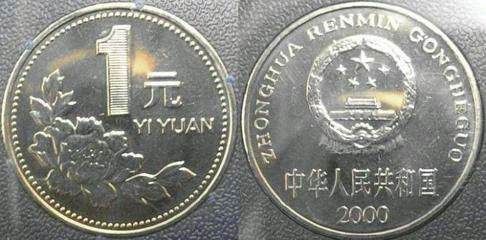
\includegraphics[width=0.4\textwidth]{figure/coin} \hspace{2cm} $\begin{bmatrix}\frac{1}{2} & 0 \\
0 & \frac{1}{2} \end{bmatrix}$

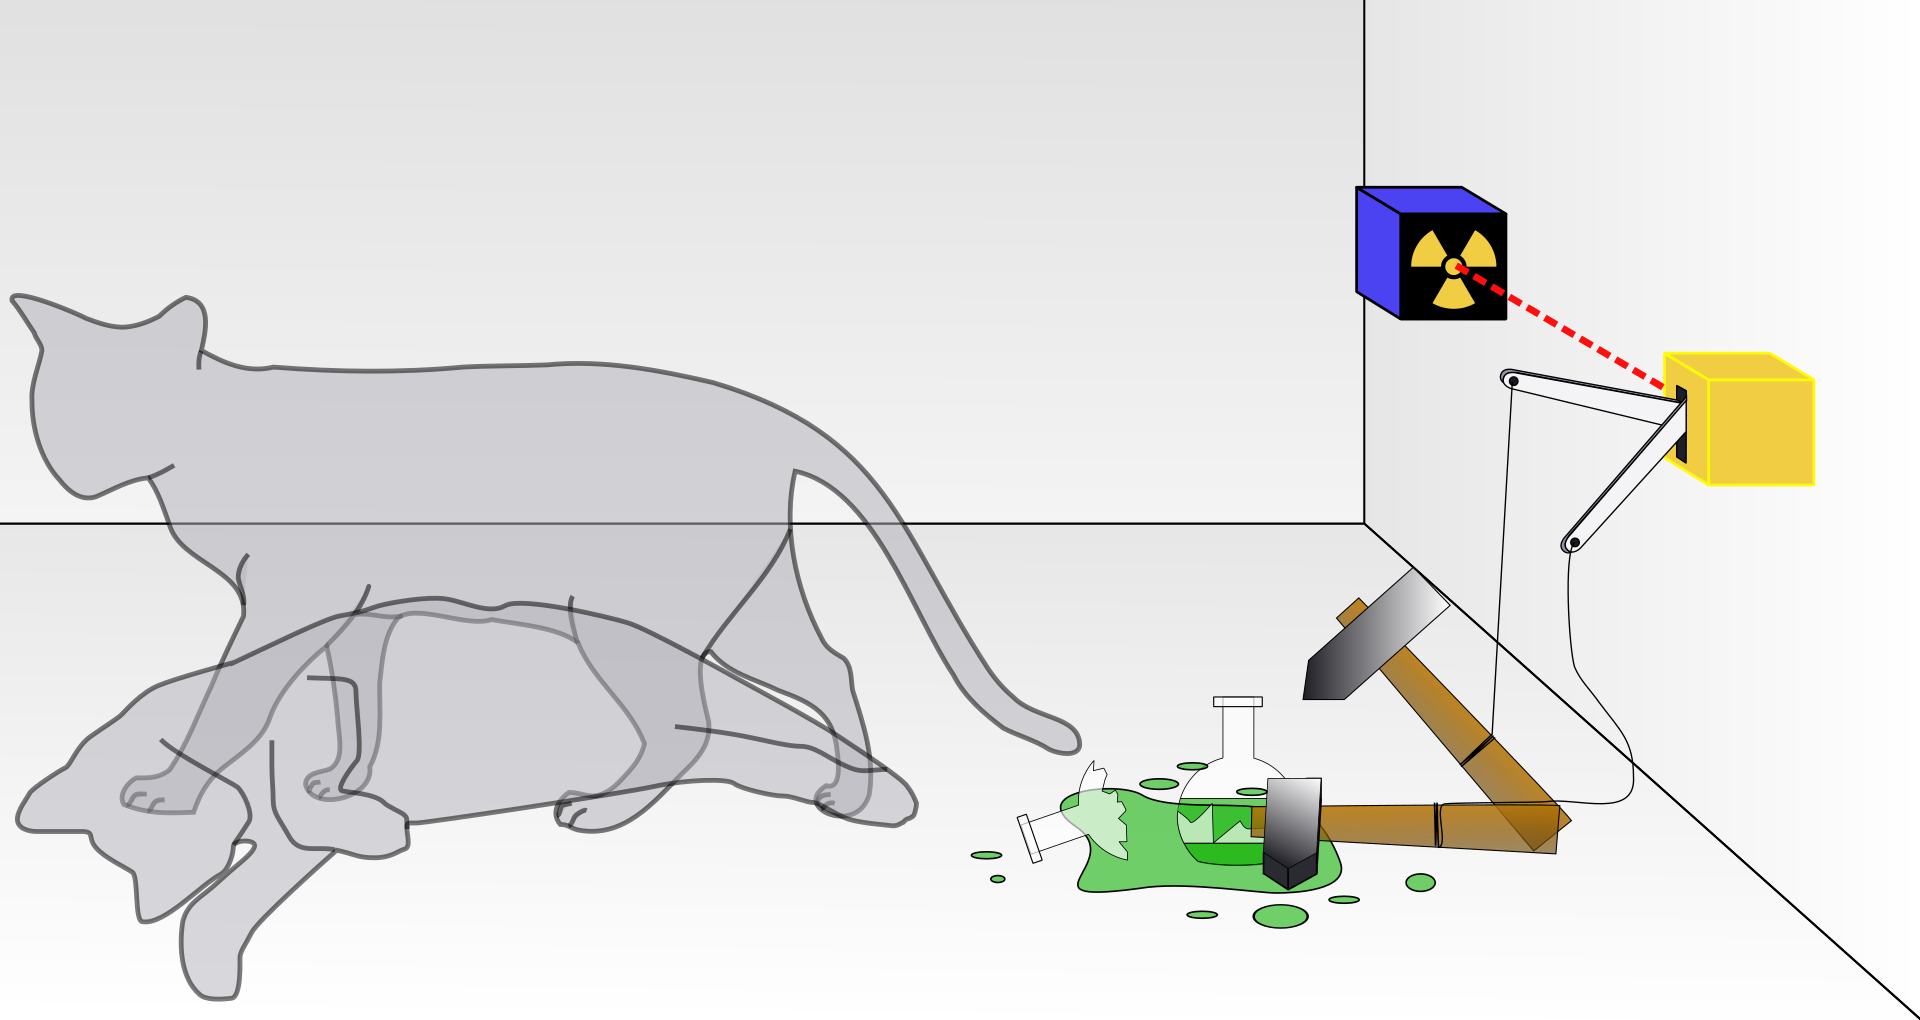
\includegraphics[width=0.4\textwidth]{figure/schrodingerscat} \hspace{2cm} $\begin{bmatrix}\frac{1}{2} & \frac{1}{2} \\
\frac{1}{2} & \frac{1}{2}\end{bmatrix}$

\vspace{1cm}

\textsc{\Large 科学在于给这个世界寻找合适的数学结构}\\[0.5cm]

\textsc{\Large 学习数学建模需要通过欣赏、临摹和实践}\\[0.5cm]
	
\textsc{\Large Teach Less, Learn More}\\[0.5cm]
	
\vfill

% Bottom of the page
{\large \today}

\end{center}
\end{titlepage}

\tableofcontents


%\chapter*{序}
%\begin{center}
%留给裴老师的地方。
%\end{center}


\chapter*{献给}
\begin{minipage}[l]{0.3\textwidth}
\hspace{4cm}
\end{minipage}
\begin{minipage}[l]{0.25\textwidth}
	我的夫人冯倩,女儿吴立心、吴逸兮
\end{minipage}
                
     
\chapter*{致谢}
在这里感谢老师、学生、家人

本书的电子版可以从网页\href{http://www.systemsci.org/jinshanw/books}{“吴金闪的书们”}找到。如果你是实体书的读者,需要输入网址的话,它是:\href{http://www.systemsci.org/jinshanw/books}{http://www.systemsci.org/jinshanw/books}。

\chapter*{前言}

%\begin{figure}
%\begin{center}
%\includegraphics[width=11cm]{figure/QuantumBook}
%\caption[本书结构图]{本书的体系结构和大多数书不太一样,对于为什么量子系统的理论形式必须是基于矢量叠加原理的量子力学做了很多的讨论。因此,量子系统的实验行为部分在本书里面也占了很大的篇幅,而理论部分从“密度分布函数”到“密度矩阵”的转变以及转变的原因占了核心的地位。通过这样的结构,我们希望读者除了了解量子力学是什么之外,还能够思考为什么量子力学会这样并对此形成一定的理解。图中的下半部分是一个总结,请读者把它和上半部分联系起来,比如通过思考“例如”的关系:“数学结构”——“例如”——“矢量空间”。}
%\FigLabel{fig:QuantumBook}
%\end{center}
%\end{figure}

\part{引论:什么是数学模型和数学建模}
科学家,尤其是物理学家,其主要目的就是给实际的世界提供一个可计算的可证伪的\footnote{一个理论其所推导出来的结果原则上可以被实验和实践证明是错的,但是迄今为止,还没有被证明是错的就叫做可证伪的但是尚未被证伪的理论。更加深入的讨论见\cite{Popper:Logic}}理想模型,通过对这个理想模型做计算,人们能够得到实际世界的行为。

\chapter{从七桥问题到图论和网络}
\ChapLabel{Chap:Graph}
在这一章里, 我们看看,图论是如何受现实世界的启发而发展起来的,以及后来发展成了什么样的进一步的描述世界的数学结构。


\section{奇偶分析和一笔画,图论初步}
网络科学是从图论发展过来的,而图论据说起源于一个称为“哥尼斯堡(Königsberg)七桥问题”的一笔画问题。

在哥尼斯堡(Königsberg)有七座桥联通四块陆地,如图\FigRef{Fig:Konigsberg}所示。哥尼斯堡(Königsberg)的人们提出了一个智力游戏,问,如果有人希望在散步的时候把每座桥都走并且只走一遍,请你给他设计一个走的方案。这个问题被称为\gls{term:Königsberg七桥问题}。

\begin{figure}
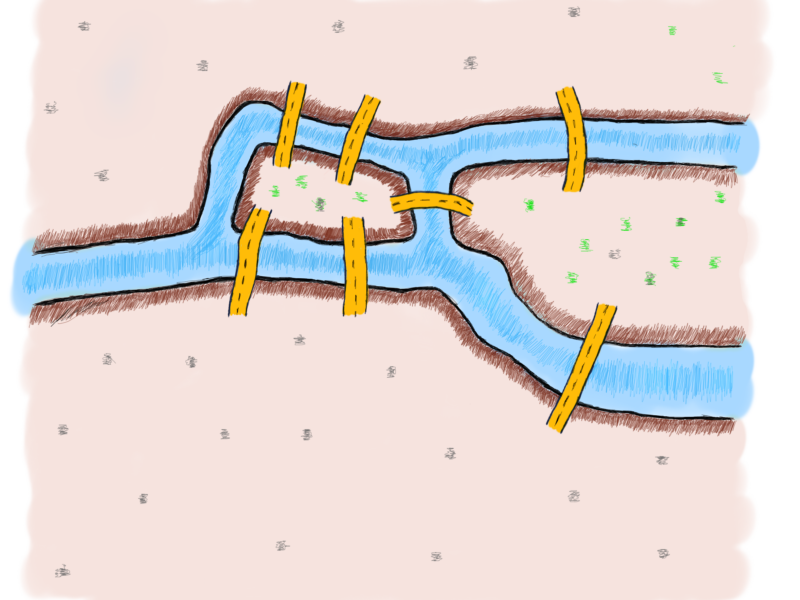
\includegraphics[width=13cm]{figure/Konigsberg.png}
\caption[Königsberg 七桥问题]{Königsberg的 七座桥联通了两条河流分割出来的四块陆地。有一个很闲的人,希望在散步的时候把每座桥都走并且只走一遍,请问他要怎么走?\remark{图按照这张以及wikipedia上的,重新制作。}}
\FigLabel{Fig:Konigsberg}
\end{figure}

\begin{figure}
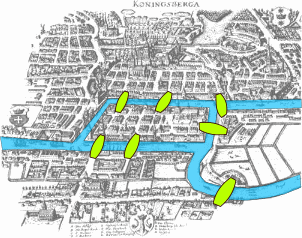
\includegraphics[width=13cm]{figure/Konigsberg2.png}
\caption[Königsberg 七桥问题]{Königsberg的 七座桥联通了被两条河流分割出来的四块陆地。有一个很闲的人,希望在散步的时候把每座桥都走并且只走一遍,请问他要怎么走?\remark{或者直接用wikipedia版本也行,则需要做如下的致谢:图片来自于Wikipedia“Seven Bridges of Königsberg”词条,原作者Bogdan Giuşcă,此图的分享遵循原作者选择的“\href{https://creativecommons.org/licenses/by-sa/3.0/deed.en}{Creative Commons Attribution-Share Alike 3.0 Unported}”协议。}}
\FigLabel{Fig:Konigsberg2}
\end{figure}

数学家\gls{name:Euler}解决了这个问题:证明不存在这样的过且仅过哥尼斯堡(Königsberg)的每一座桥一次的走法,并且把这个问题推广成了任意的有顶点和连边构成的图是否可以一步画的判定定理。下面我们学着\gls{name:Euler}来解决一下这个问题。这一小节的资料主要来自于\href{https://en.wikipedia.org/wiki/Seven\_Bridges\_of\_K\%C3\%B6nigsberg}{Wikipedia“Seven Bridges of Königsberg”词条}\footnote{https://en.wikipedia.org/wiki/Seven\_Bridges\_of\_Königsberg,\today 访问。}以及\gls{name:姜伯驹}的《一笔画和邮递路线问题》\cite{Hua:Collection}。

首先,\gls{name:Euler}注意到,在每一块陆地之内怎么散步跟这个问题没关系。于是,每一块陆地都可以看做一个点,从而忽略陆地的细节,以及连接同一块陆地上的多座桥是否在同一个地点连接的问题。我们把陆地分解标记为SCEN,其中$S$代表南边的陆地,$C$代表中间的陆地,$E$代表东面的陆地,$N$代表北面的陆地。现在,我们把每个区域看做一个点,主要留下每一对区域之间有几座桥这个信息,就得到了简化了的图\FigRef{Fig:Konigsberg4}。

\begin{figure}
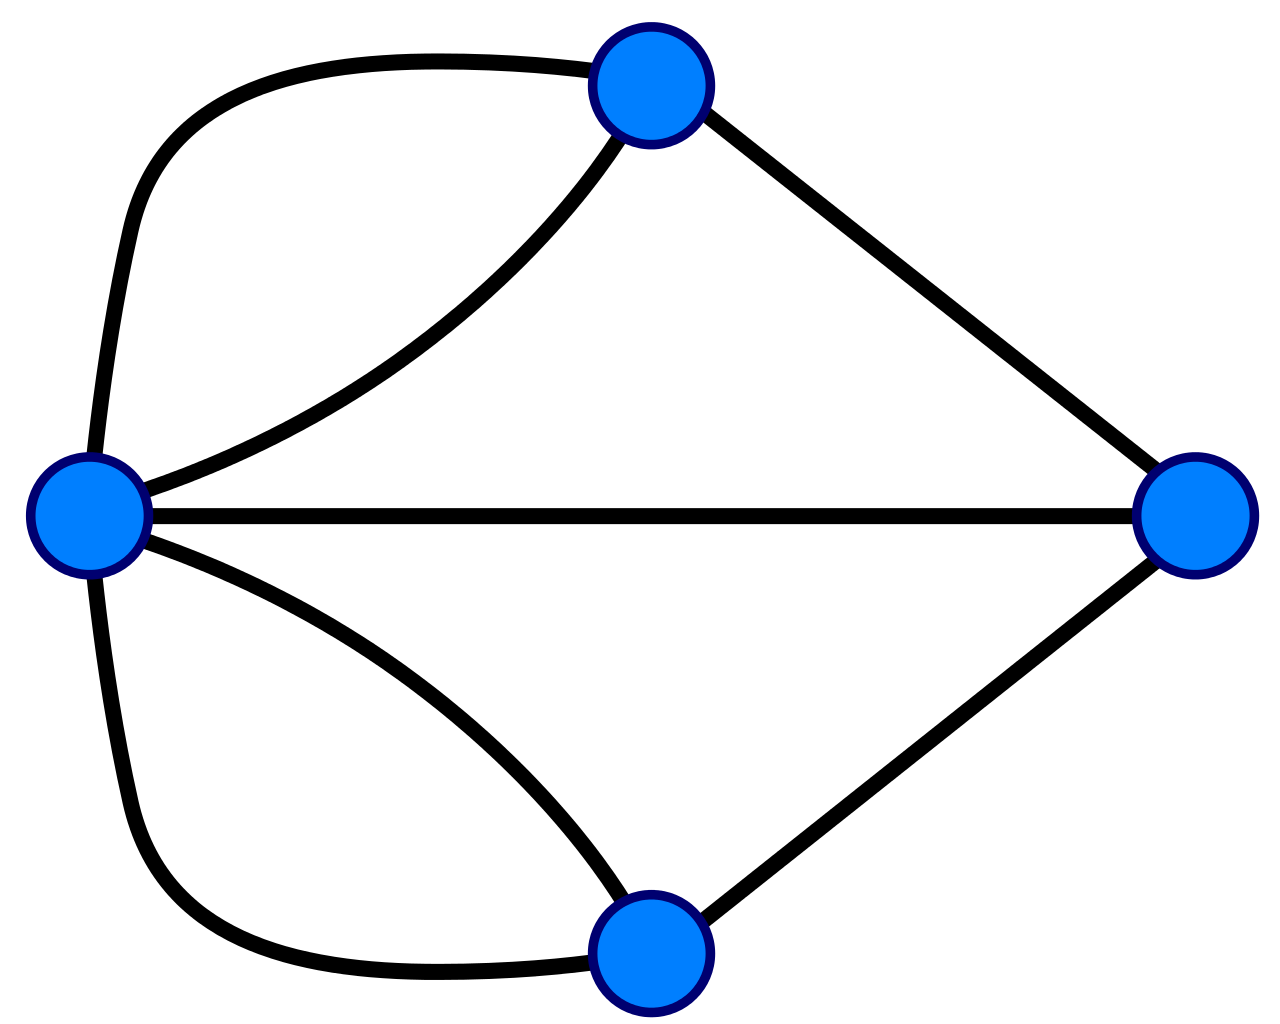
\includegraphics[width=13cm]{figure/Konigsberg4.png}
\caption[Königsberg 七桥问题示意图]{把Königsberg的每块陆地变成一个点,保留任意两个点之间有几座桥的信息,得到的简化图。\remark{图重新做,加上SCEN的标记。}}
\FigLabel{Fig:Konigsberg4}
\end{figure}

我们发现,$S$区域有三座桥和其他区域相连(分别是$SC, SC, SE$),$C$区域有五座桥和其他区域相连(分别是$CS, CS, CN, CN, CE$),$E$区域有三座桥和其他区域相连(分别是$ES, EC, EN$),$N$区域有三座桥和其他区域相连(分别是$NC, NC, NE$)。现在,原始的每座桥走且仅走一次的散步计划的问题,就成了一笔画问题:在由顶点和连边构成的图上,需要放下和拿起来笔一次中间不能再次拿起来从其他地方重新开始,连续地把所有的连边都画并且仅仅画一次。

接着,对于这个一笔画问题,\gls{name:Euler}发现,除了当做开始和结束的顶点(称为起点和终点,它们也可以是同一个顶点),其他顶点必须经过偶数次。为什么呢?因为一笔画的时候,除了起点和终点,都必须进去以后在出来,而且每一次进去就对应着一次出来。由于每一次进出必须用到一条边,而且这条边还必须和之前的边不同,因此,这也就意味着,一笔画的时候,除了起点和终点的其他顶点必须有偶数条边和其他顶点相连。我们把一个顶点的连到其他顶点的边的数量称为这个顶点的度。于是,如果可以一笔画,则这个图除了起点和终点,其他顶点的度必须是偶数。

再来考虑起点和终点。如果起点和终点不相同,则可以允许它们的度为奇数。例如,一条线直接把两个顶点相连,这能够一笔画,起点和终点的度都是$1$,奇数。如果起点和终点相同,则这个顶点既进又出,每次进出也同样必须有两条连边,因此这个顶点的度是偶数。也就是说,对于一笔画来说,我们可以有$0$个或者$2$个度为奇数的顶点。

合起来,我们得到
\begin{Theorem}
{一笔画问题的必要条件}{}由顶点和连边构成的图,可以一笔画的必要条件(必须满足下面的条件才可能一笔画出来)是,图是连同的,有$0$个或者$2$个度为奇数的顶点,其他的顶点的度都是偶数。
\end{Theorem}
我们用这个条件来看一下Königsberg 七桥问题:连通\footnote{将来,我们还会学习到甚至自己来构建判断连通性的更简单的算法,目前,你只能通过来试试,是否从任意一个顶点开始都可以走到任意另一个顶点上去。},但是$S、C、E、N$的度分别是$3$、$5$、$3$、$3$,四个奇数度的顶点不满足要求,因此不能一笔画,也就是不存在每一座桥经过而且只一次的散步路线。

实际上,\gls{name:Euler}还猜测,这个必要条件是充分条件,也就是
\begin{Theorem}
{一笔画问题的充分条件}{}由顶点和连边构成的图,如果是连通的,并且有$0$个或者$2$个度为奇数的顶点,其他的顶点的度都是偶数,则肯定可以一笔画出来。
\end{Theorem}
这个定理由数学家\gls{name:Hierholzer}证明,并且\gls{name:Hierholzer}还给出了一笔画的算法\footnote{这个算法就被称为Hierholzer算法。有兴趣的可以去进一步了解。},也就是回答了一旦满足这个条件,如何把一笔画的顺序找出来的问题。充分条件的定理的证明我们就不在这里展开了。

我们看到,通过把是否可以一笔画的问题和怎么来做一笔画的问题分开,并且把问题归结为顶点的度的计算的问题,我们得到了非常容易的判断一张图是否可以一笔画的条件。

一笔画问题是巧妙运用奇偶分析来解决问题的一个例子。奇偶分析是一个非常具有一般性而且有威力研究问题的角度。将来在\SecRef{Sec:irrational}和\SecRef{Sec:Contradiction},我们还会用它来证明一个自己跟自己乘起来等于$2$的数\footnote{这个数满足$a\times a =2$。将来,我们会把它记做$\sqrt{2}$。}不是分数。

前面的一笔画问题的解决过程还体现了抽象——把具体的包含多个属性大量细节的对象变成更加具有一般性的往往还更加简单的包含更少属性和细节的对象,同时保证解决了这个更简单更一般的对象的问题之后可以回来解决那个更具体的对象上的问题——在数学思维中的重要性。如果Euler不去忽略每个岛的细节而把问题变成了仅仅包含“顶点”和“连边”的对象的问题,那一笔画的问题就不可能被Euler这样解决,或者说,至少就算能解决也仅仅解决了 \gls{term:Königsberg七桥问题},而不能用于其他类似的问题。正是由于这个对一笔画问题的抽象实在太深刻而成功了,因此,后来以此为基础还发展出来两个数学分支学科:一个叫做图论或者后来称为网络科学,一个是拓扑学。

前面的一笔画问题的解决过程还体现了“把存在性证明和找算法这两步分开”,甚至在任何本来是寻找算法的问题中,尽量先尝试存在性证明,这个数学思维的力量。如果Euler不去思考解的存在性,而是一直关注如何画图,也就是求解问题,那一笔画的问题就不可能被Euler这样解决。

\section{推荐阅读材料}
推荐阅读吴军的《数学之美》\cite{Wu:MathBeauty}和\gls{name:Gowers}的《牛津通识读本:数学》。


\section{作业}
\begin{Homework}			
阅读\gls{name:Gowers}的《牛津通识读本:数学》\cite{Gowers:Math},并做读书报告,回答:说了什么,怎么说的,为什么这样说为什么说这个,我觉得怎么样也就是对我有什么意义。
\end{Homework}


\chapter{经典力学和微积分}
\ChapLabel{Chap:Calculus}
在这一章里, 我们看看,微积分是在什么样的背景下提出来的,是为了描述和解决什么问题的。当然,微积分的完善是纯数学基础数学的研究问题,但是,它的提出其实是一个数学建模,至少从Newton的角度。

\section{作业}
\begin{Homework}			
阅读\gls{name:Bender}的《数学模型引论》\cite{Bender:MathModel},并做读书报告,回答:说了什么,怎么说的,为什么这样说为什么说这个,我觉得怎么样也就是对我有什么意义。
\end{Homework}



\section{本章小结}


\chapter{量子力学和矢量代数}
\ChapLabel{Chap:Vector}

在这一章里, 我们看看量子系统为什么用Hilbert空间的矢量和算符来描述。在这个问题上,数学走在了物理学的前面。有的时候,物理学的现象和概念使得数学的概念得到提出和发展。有的时候,数学的概念在物理学里面得以发挥作用。
\section{典型经典随机现象和经典随机描述}
\section{典型量子现象}
\begin{figure}
\begin{center}
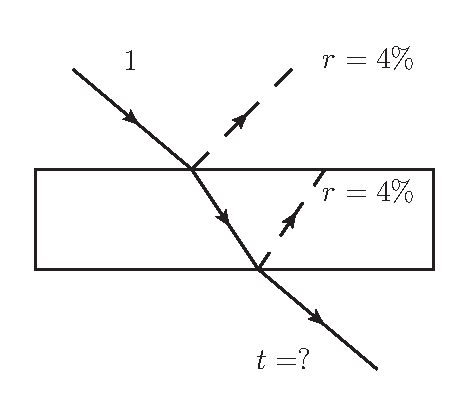
\includegraphics[width=6cm]{figure/GlassReflect.eps}
\caption[Feynman的光过玻璃示意图]{光子经过一块玻璃,可以在玻璃的两个界面上发生反射和透射。那么从第一个界面出来的光就可能是第一次反射形成的,也可能是第一个界面和第二个界面反射并且在第一个界面透射以后形成的。这样互斥事件形成的光能够相互抵消吗?如果不能,我们给相机镜头镀膜——这里把膜看作新的一层玻璃——干什么?}
\FigLabel{fig:GlassReflect}
\end{center}
\end{figure}

\begin{Experiment}
[相机镜头上的贴膜形成的光的干涉现象]:镜头上的贴膜就是让光尽可能多地通过镜头之前的膜而不是被这个膜反射太多\cite{Moghal:Antireflection},然后,也降低在膜和镜头——可以是玻璃或者塑胶——之间的反射。现在,我们来关心前半部分——如\FigRef{fig:GlassReflect}所示的光过膜的两个界面——的过程。为了简单起见,我们用Feynman在《QED: The Strange Theory of Light and Matter》\cite{Feynman:Strange}中的光过玻璃的例子——把光过贴膜改成光过玻璃。概念上两者没有区别。
\end{Experiment}

\begin{figure}
\begin{center}
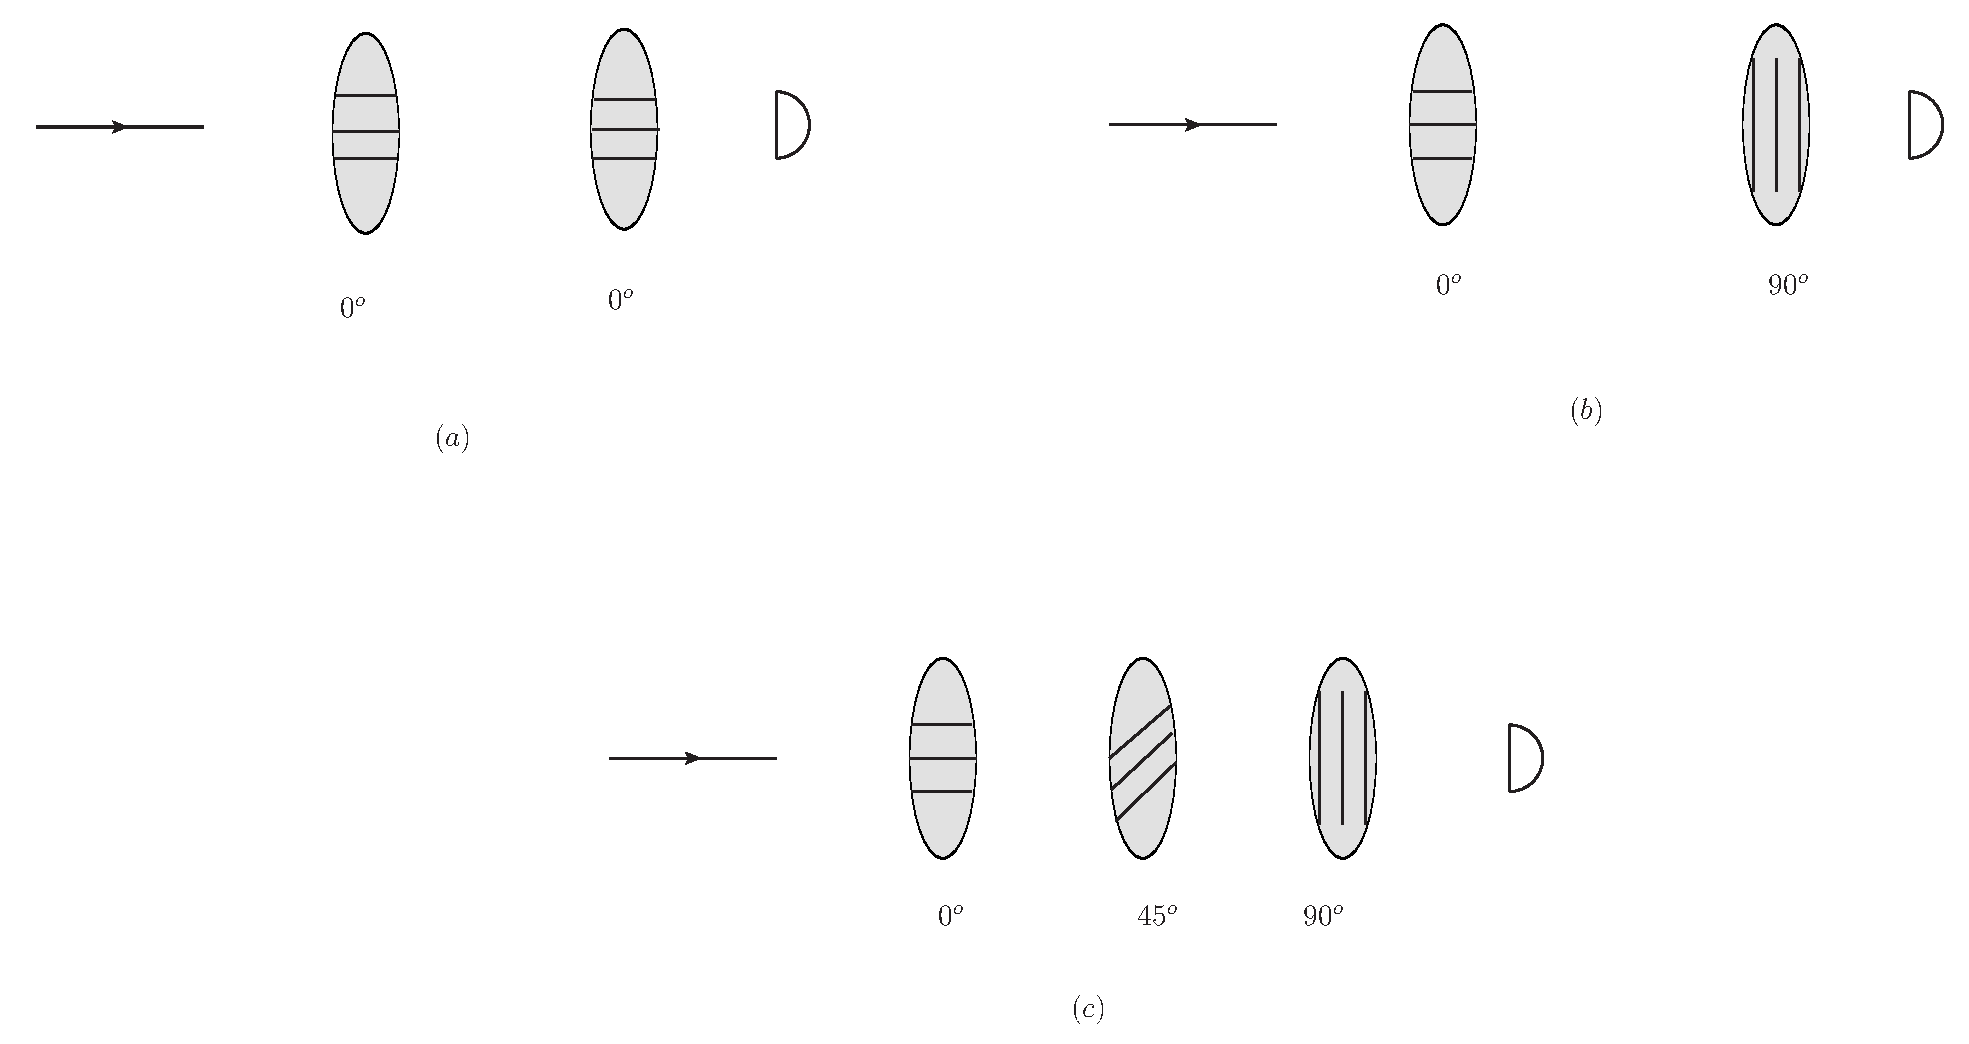
\includegraphics[width=8cm]{figure/Dirac3Polar}
\caption[Dirac的光三块偏振片]{(a).光过两块平行偏振片(透过)。(b).光两块垂直偏振片(挡住)。(c).光过三块偏振片——最前最后两块相互垂直,中间的偏振片处于前后两者之间的某一角度(透过)。}
\FigLabel{fig:Dirac3Polar}
\end{center}
\end{figure}

\begin{Experiment}
[\gls{term:Dirac的光过三块偏振片}]:找三块完全相同的偏振片来做如\FigRef{fig:Dirac3Polar}所示的三个实验。先拿其中的两块做实验$A$:一手拿一块偏振片,把两块偏振片完全平行地放在面前,透过镜片看物体。观察是否能够看到东西,还是基本不能透光?再拿这两块做实验$B$:一手拿一块偏振片,把两块偏振片垂直地放在面前,透过镜片看物体。观察是否能够看到东西,还是基本不能透光?接着取出第三块镜片,做实验$C$:把第三块镜片以某个角度——与之前的镜片都不平行——插入到实验$B$的两块之间(这时候你可能需要别人帮忙)。观察是否能够看到东西,还是基本不能透光?

实验结果是:$A$通过两个平行镜片看物体,基本上没变(光的强度有变化,但是能够清楚地看到镜片之后的物体);$B$通过两个垂直镜片看物体,基本上看不到镜片之后的物体;$C$增加一个镜片以后,之前不能看到的镜片之后的物体又能够看到了。
\end{Experiment}

\begin{figure}
\begin{center}
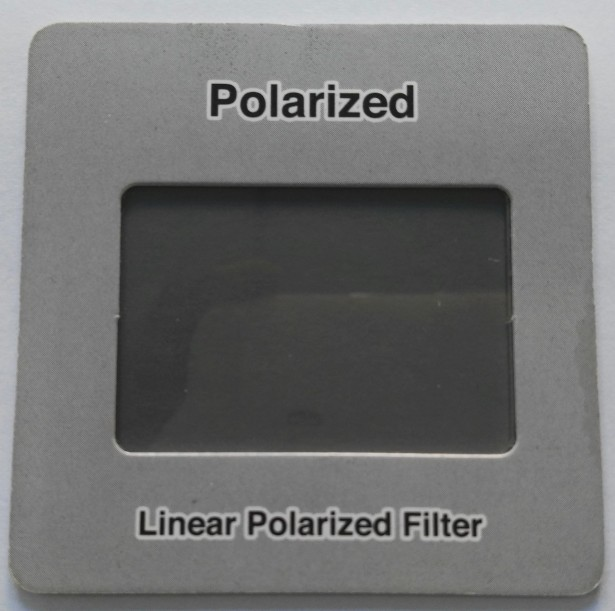
\includegraphics[width=6cm]{figure/Polarizer.jpg}
\caption[便宜的偏振片]{这个偏振片专门是开发了做教具的,非常便宜。}
\FigLabel{fig:Polarizer}
\end{center}
\end{figure}
这个(将来我们会看到的)量子效应如此显著的实验,竟然是可以在家里做的,只要购买三个偏振片,例如偏振墨镜或者如\FigRef{fig:Polarizer}的教具。

\begin{figure}
\begin{center}
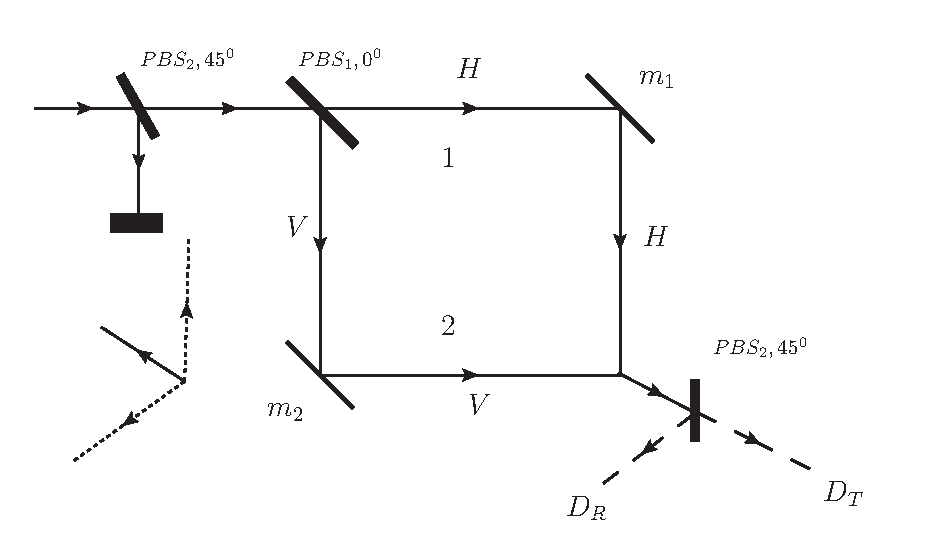
\includegraphics[width=6cm]{figure/QMPBS.eps}
\caption[光子which-way实验装置示意图]{光子which-way实验装置示意图。其中最后一步把两个不同路径来的光又合起来然后进入偏振分束器在实验中需要一个额外的仪器来完成。在这个示意图里面我们只需了解能够做到这样的合起来就可以了。注意偏振分束器的内部方向和图中的仪器的摆放方向不是一个东西。}
\FigLabel{fig:QMPBS}
\end{center}
\end{figure}

\begin{Experiment}
[光子which-way实验]:如\FigRef{fig:QMPBS}所示,一个光子经过第一面内部方向为$45^{0}$(见图中所示的坐标系)偏振分束器之后,只允许透射光过去,反射光被完全挡住。然后这个光子继续经过一个$0^{0}$的偏振分束器。经过这个分束器的光子可能走两条路径。不管走哪一条,它都会被反射会到同一个位置(右下角),然后被引入到第三个内部方向为$45^{0}$偏振分束器。问:分束器之后的探测器$D_{T}$和$D_{R}$上都会有接收到光子的可能吗?

这个实验的结果\footnote{实际的实验在最后一步探测的不是“哪一个方向上有粒子”,而是探测是否两个路径上过来的粒子“是否会出现干涉条纹”\cite{Lukishova:Rochester}。如果有干涉条纹则表示路径信息消失了,就不能问“粒子到底从哪一条路上过来”了。}是只有$D_{T}$上有光子到达。
\ExpLabel{exp:photonwhichway}
\end{Experiment}
\begin{figure}
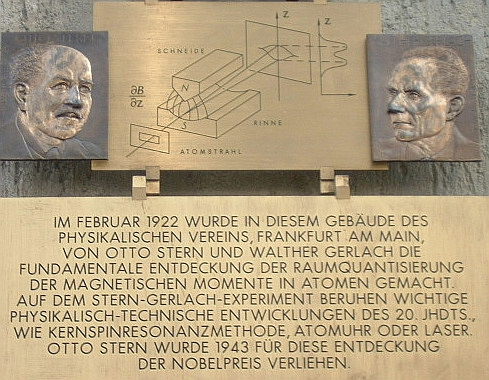
\includegraphics[width=12cm]{figure/SternGerlach2}
\caption[自旋的Stern-Gerlach装置]{来自于\gls{name:Stern}和\gls{name:Gerlach}的自旋\gls{term:Stern-Gerlach装置}示意图。图片来自于Wikipedia页面\url{https://en.wikipedia.org/wiki/Stern-Gerlach_experiment}。}
\FigLabel{fig:SternGerlach}
\end{figure}

\begin{figure}
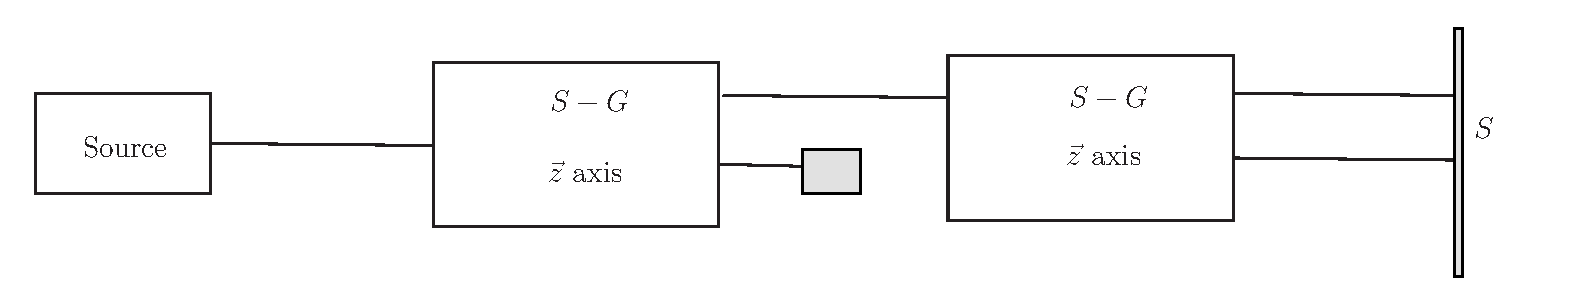
\includegraphics[width=12cm]{figure/SG.eps}
\caption[自旋过Stern-Gerlach装置示意图]{自旋经过一个Stern-Gerlach装置——其内部就是一个磁场——之后挡住向下的输出,这样从装置出来的状态就是第一个装置的向上方向。接着让这个输出的自旋再一次经过同样方向的装置——得到仅有一个向上的输出结果。}
\FigLabel{fig:SGSzSz}
\end{figure}

\section{量子现象的数学描述}
为什么要有矢量加法,为什么要有非对易算符

\chapter{毛皮贸易及其背后的捕食者-被捕食者模型}
\ChapLabel{Chap:Lotka-Volterra}

\chapter{第一部分总结:什么是数学模型和数学建模}
\ChapLabel{Chap:Part1}

\part{数学建模的典型思维方式}

\chapter{假设的提出修改和精炼}
\ChapLabel{Chap:Assumption}
抓住主要矛盾,简化,冲着某个目标,不断地挑战和修订假设,不断地思考计算的意义和条件

\chapter{数学基础和学习的问题}
\ChapLabel{Chap:Basis}
画画,先学会技巧,还是先学会表达,能一起学吗?写作,先有思想,还是现有先做技巧,能一起有吗?

学习数学,需要回到概念和计算提出来的场景下。

数学就是需要的时候,我去创造它。如果已经被创造,那就算别人的,我就用好它。

\chapter{系统图示法}
\ChapLabel{Chap:Diagram}
一切在于联系,内部、外界

量纲分析:确定有哪些因素的意义

系统科学
\chapter{第二部分总结:大概如何数学建模}
\ChapLabel{Chap:Part2}

\part{数学建模赏析和练习}

\chapter{连续状态动力学过程的建模的几个例子}
\ChapLabel{Chap:DE}
动力学方程的思想——状态、状态演化和技术——微分方程模型

\chapter{离散状态动力学过程的建模的几个例子}
\ChapLabel{Chap:Markov}
Markov过程

\chapter{粗糙的数学问题集以及少量提示}
\ChapLabel{Chap:Questions}
关键在于尝试、练习和指导

\chapter{第三部分总结:再一次问如何数学建模}
\ChapLabel{Chap:Part3}

\chapter*{结束语}
整本书到此结束。本书在内容选择甚至具体内容的展开上都和大多数书不太一样。希望这个企图做到不一样的努力能够对于学习者的学习和理解有点效果(make a difference)。 

内容上贯穿全书的是从什么是数学模型什么是数学建模——为现实世界找到忠实或者近似忠实的数学表示。

谢谢你作为学习者付出的时间和努力,希望你喜欢这个深入思考的过程。

%\bibliographystyle{GBT7714-2005N} %多作者会出问题
%\bibliographystyle{gbt7714-2005} %多作者会出问题,全大写,愚蠢的GB标准,当有西班牙与字符的时候
\bibliographystyle{buptthesis} %好用
%\bibliographystyle{GBT7714-2005NLang-UTF8} %全大写,愚蠢的GB标准,当有西班牙与字符的时候
\bibliography{MathModel}
\addcontentsline{toc}{chapter}{参考文献}

\printglossary[type=term]
\printglossary[type=name]
\addcontentsline{toc}{chapter}{插图目录}
\listoffigures
\renewcommand{\listtheoremname}{举例}
\listoftheorems[ignoreall,show={Example}]
\addcontentsline{toc}{chapter}{举例目录}

 \end{document}
